% THIS IS SIGPROC-SP.TEX - VERSION 3.1
% WORKS WITH V3.2SP OF ACM_PROC_ARTICLE-SP.CLS
% APRIL 2009
%
% It is an example file showing how to use the 'acm_proc_article-sp.cls' V3.2SP
% LaTeX2e document class file for Conference Proceedings submissions.
% ----------------------------------------------------------------------------------------------------------------
% This .tex file (and associated .cls V3.2SP) *DOES NOT* produce:
%       1) The Permission Statement
%       2) The Conference (location) Info information
%       3) The Copyright Line with ACM data
%       4) Page numbering
% ---------------------------------------------------------------------------------------------------------------
% It is an example which *does* use the .bib file (from which the .bbl file
% is produced).
% REMEMBER HOWEVER: After having produced the .bbl file,
% and prior to final submission,
% you need to 'insert'  your .bbl file into your source .tex file so as to provide
% ONE 'self-contained' source file.
%
% Questions regarding SIGS should be sent to
% Adrienne Griscti ---> griscti@acm.org
%
% Questions/suggestions regarding the guidelines, .tex and .cls files, etc. to
% Gerald Murray ---> murray@hq.acm.org
%
% For tracking purposes - this is V3.1SP - APRIL 2009

\documentclass{acm_proc_article-sp}

\begin{document}

\title{Prototype of an event-driven Future Internet Cockpit -  Real-Time Sensor Events for Complex Event Processing}
% \subtitle{[Event processing]}

%
% You need the command \numberofauthors to handle the 'placement
% and alignment' of the authors beneath the title.
%
% For aesthetic reasons, we recommend 'three authors at a time'
% i.e. three 'name/affiliation blocks' be placed beneath the title.
%
% NOTE: You are NOT restricted in how many 'rows' of
% "name/affiliations" may appear. We just ask that you restrict
% the number of 'columns' to three.
%
% Because of the available 'opening page real-estate'
% we ask you to refrain from putting more than six authors
% (two rows with three columns) beneath the article title.
% More than six makes the first-page appear very cluttered indeed.
%
% Use the \alignauthor commands to handle the names
% and affiliations for an 'aesthetic maximum' of six authors.
% Add names, affiliations, addresses for
% the seventh etc. author(s) as the argument for the
% \additionalauthors command.
% These 'additional authors' will be output/set for you
% without further effort on your part as the last section in
% the body of your article BEFORE References or any Appendices.

\numberofauthors{1} %  in this sample file, there are a *total*
% of EIGHT authors. SIX appear on the 'first-page' (for formatting
% reasons) and the remaining two appear in the \additionalauthors section.
%
\author{
% You can go ahead and credit any number of authors here,
% e.g. one 'row of three' or two rows (consisting of one row of three
% and a second row of one, two or three).
%
% The command \alignauthor (no curly braces needed) should
% precede each author name, affiliation/snail-mail address and
% e-mail address. Additionally, tag each line of
% affiliation/address with \affaddr, and tag the
% e-mail address with \email.
%
% 1st. author
\alignauthor
Robin B\"ohm\\
       \affaddr{University of Duisburg Essen}\\
       \affaddr{paluno - The Ruhr Institute for Software Technology}\\
       \affaddr{Sch\"utzenbahn 70, 45117, Essen, Germany}\\
       \email{robin.boehm@stud.uni-due.de}
}

\maketitle
\begin{abstract}
In this user study we challenge the problems that occurs in the logistic sector in combination with the transport process of perishable goods.
It treats the problems about providing, receiving and processing information in real-time to improve the reaction time issues.

We developed a prototype architecture for an event-driven cockpit with the ideas of the Future Internet(FI). It is about monitoring our business case of transporting perishable goods in the logistic domain with concepts of Internet of Things (IoT). 
It uses a service platform that provides sensor event data for things in the real-wold that are provided via the websocket protocol - this platform based on the 
These events are aggregated and interpreted by an Complex Event Engine(CEP) and visualized via an cockpit in a web-browser.
Through the chosen architecture the latency between the actual business event and the visualization is nearly real-time and gives an additional benefit to the existing solutions.
\end{abstract}


\section{Introduction}
The transport of perishable goods in the logistic sector is a challenging task. It deals with a huge amount of data and real-time data processing.
The current development of some state-of-the-art Future Internet(FI) technologies shows a great potential to improve this business processes.

The chosen use-case is a business process management in the logistic sector that handles  perishable goods. To manage this task it is necessary to manage trucks, routes and have an overview about the current state of the deliveries. We focused on the task of reducing the latency between the actual business event and the delivery of the information to improve the possibility to react quickly to this events and increase the value of this information as shown by Hackathorn\cite{hackathron:real_time_to_real_value}.

We are using the Internet of Things(IoT) and Internet of Services(IoS) concepts to linking the real-world with our business world. So we are able to use real-time sensor events to create our virtual model. We are able increase the amount and quality of event-data that can be used for calculations and combine them to more valuable complex events.
To handle the messaging inside of our prototype we decided to use an Event-driven-Architecture(EDA) in combination with an Complex-Event-Processing(CEP) Engine to defining the rules for our complex events.

We are providing a cockpit for monitoring the business model with some useful visualizations.This cockpit is implemented with modern web technologies so it is usable on many devices out of the box over the specifications. It contains a map that shows the current state of given routes with an rating calculated on the raw events. Also a table that offers information in more textual way.

\begin{figure}[h]
	\begin{center}
		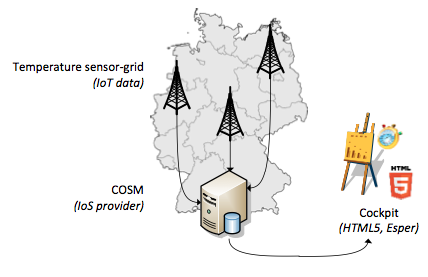
\includegraphics[scale=0.5]{overview.png}
		\caption[Project overview]{Project overview}
		\label{fig:Project overview}
	\end{center}
\end{figure}

This paper starts with an introduction about the basics in section \ref{sec:Basics}.
After a survey of related work in Section \ref{sec:Related Work}. 
The Use-Case is described in section \ref{sec:Use Case} and our design considerations of the different components are part of section \ref{sec:Conceptional Design}.
The next section \ref{sec:Implementation} contains details about the implementation with a technical stack component overview followed by the conclusion in section \ref{sec:Conclusion}.

\section{Basic}
\label{sec:Basics}

The idea of \textbf{Future Internet} is to enhance the architectures for the current state of the Internet. There are many ideas that are elaborated and discussed. It is a superset of different paradigms and developments. 
One of the most interesting ideas is defined by the \textbf{Internet-of-Things} term that first used by Kevin Ashton in the year 1999 \cite{•}. He describes the IoT as enhancement from human-entered data to real world data that is captured by machines.
\begin{quote}
If we had computers that knew everything there was to know about things - using data they gathered without any help from us - we would be able to track and count everything, and greatly reduce waste, loss and cost. We would know when things needed replacing, repairing or recalling, and whether they were fresh or past their best. \cite{iot_thing:Ashton}
\end{quote}
So IoT can described as global sensor network of object and things that providing information about their current state. This is a big deal for informational processing and could be used in very different ways, for example to improve business processes.
There is another concept of FI that could enables us to use all this information that is called \textbf{Internet of Services}. This is a concept that describes next-generation services that are world-wide available and could be used. They are highly adaptive and can be integrated in own services \cite{future_Internet:shenker}.
A service platform that is named COSM and described itself as `Internet of Things Platform' on the website\cite{cosm} is implementing this kind of idea. This platform enables developers and companies to connect devices and exchange data over an defined API that use the websocket protocol.
It acts as gateway between the connected sensor devices and the consumer that using this information via the api.

To handle this high amount of realt-time data in information systems is likely to use an \textbf{event-driven-architecture} (EDA). An EDA is defined as one that has the ability to detect events and react intelligently on them. Also its designed to handle real-time or nearly real-time changes in business conditions.\cite{EDA:Taylor}

To add some more more meaningful value for some special business case \textbf{Complex Event Processing}(CEP) can be used. CEP is a method that tracks and analyses events and combine them to more valuable complex events. A complex event can be defined through rules and combined, integrate or aggregate other events. Also temporal rules can be defined that detecting the occurrence of events in a defined time interval.

\section{Related Work}
\label{sec:Related Work}

The term Internet of Things exists in the Context of Future Internet now about ten years. 
So many papers where published that deals with this topic.
A good introduction into the Internet of Things Vision is given by Vermesan in his research roadmap. At the beginning he describe the Future Internet version with all the paradigms that exists in this category\cite{vermesan2009internet}. Later he focus on the Internet of Things paradigm and explain some current developments and mentioned about technological trends.
He also talks about the current analyses of a European Commission estimate that it would be 16 billion connected IoT devices in the year 2020\cite{sundmaeker2010vision}.

In the article from Luigi Atzori he wrote a survey about enabling technologies in telecommunications, informatics and electronics. He talks about the important development of the last years like Radio-Frequency IDentification tags or mobile phones with enable us to generate unique addressing schemes for things or objects that enable us to interact and cooperate with this things\cite{atzori2010internet}.
C.Winkler from the University Duisburg Essen in Germany developed a sensor network via smartphone sensors that providing data\cite{sense-sation_winkler}.
He created a platform that manage the incoming events triggered by combination of sensors and their behavior.
This sensing platform provides a RESTFul web service that offers this sensor event information.

Jaroensutasinee used Pachube, later renamed to COSM, as cloud sensor platform in the paper of the CREON group. They collected these outputs, decide if this event may has a global  and delivered them to other services like 'Twitter' or for monitoring \cite{jaroensutasineecreon}.
This project is important because it is very similar to our project challenges.
They also using a sensor platform to aggregate data, interpreting them and make them usable notices for humans.

The FINEST Project is about researching in the transport and logistic sector. As Metzger shown at the SRII conference they using the potential of the future internet development to improve logistic control systems. They describing the work with real-time data and describing the collaboration with could- and service-based platforms to solve this problems. \cite{metzger2012predictive}


\section{Use Case}
\label{sec:Use Case}

Basically our use case is about managing the delivery of perishable goods. This is a high risk business process in the logistic domain. If some goods arriving late or there are some problems with the cooling system it is necessary to get the information of the real-world state as quick as possible to do a trade-off what could be the best action to reduce risk or costs.

Our use case comprises the planing and alternatives in escalation situations of the delivery of these perishable goods via trucks over a defined route. These trucks are equipped with sensors that provides us the monitoring data that is used for automated real-time aggregation and interpretation and share the results in a cockpit application like it is described in the Internet-of-Things(IoT) concept. 
Also the routes are equipped with sensors that enables us to monitor them.
The overview in such a business monitoring tool is modeled a cockpit with summary of meaningful information that should support the decision. 

The cockpit provides an ampel-system with the colors green, yellow and red that visualizing the current state of the routes and trucks depending on defined threshold.
Also the prototype is using complex threshold for combinations of singular states of a route or a truck that currently on this route that are also visualized in a map.
The cockpit should be available via different devices like on the computer or on smart-phone.
%Actuality of the information is one of the most valuable criterion
\section{Conceptional Design}
\label{sec:Conceptional Design}

As basic architectural design we are choosing an event-driven-architecture(EDA).
An EDA is loosely coupled and can be used for distribution and scalability of software components. Because every component could have multiple listeners for his own events or act as sender for multiple other components.
For our prototype we build service components that are loosed coupled and communicating only via events.
At first we using a connector that receives basic events from the COSM Service API.
The component connects to the API and subscribe itself to the relevant data-streams that are prepared for this demo-case.
Once the component is registered to the service-api, it receives an event via push every time a change of state appears at the data-stream. Through the static connection that happens in real-time without any overhead to create a new connection.
When the event message is arrived via the socket it get parsed and transformed into the internal event structure and directly send to the components that are listening.
A registered listener in our system for this COSM-Component Events is the Complex-Event-Processing(CEP) component.

\begin{figure}[h]
	\begin{center}
		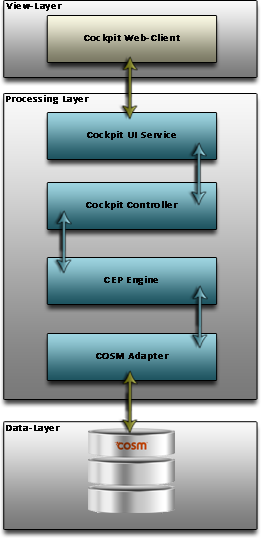
\includegraphics[scale=0.5]{Component-Overview.png}
		\caption[Component Overview]{Component Overview}
		\label{fig:AngiogeneticSwitch}
	\end{center}
\end{figure}

This component is a processing unit that is programmed with rules that results again in events. This rules are designed for the special use case of our cockpit. It forms one or many events in a temporal context to complex events that also can be the source for new rules. It is a detection for events that could be a derivation for complex events and so we adding new more valuable events than the simple events could do.
This (complex) events are used by the third component that registered as listener.
This component contains the business model. The model is updated with every event the component receives. 
To visualize this data we are providing the information as a service via a websocket api.
Our javascript client act as visualization unit that could connect to the service component and receive updates via websocket every time a state-change happens at then model site.
Through this chain of event-processing also the client receives the events triggered by the COSM-API in real-time and can provide this information for multiple clients.

\section{Implementation}
\label{sec:Implementation}

\subsection{Environment}
To mange our build process and the dependency management we used Apache Maven to handle this tasks. We provide our configuration via a xml file that defines all our  dependencies for example for the CEP components.
So the build process is automated and can be started by a simple command under different environments like Windows, Unix or Mac OS X.
To enable us to work distributed in our team we used the version control system git with a private repository at github as host
\footnote{http://www.github.com}
that provides us this as service.

Another advantage that is provided by a maven third party plugin that is named Apache Tomcat Maven Plugin
\footnote{http://tomcat.apache.org/maven-plugin.html}.
It offers a command to bundle our whole project to an jar that starts all our services with one command and can be offered as single executable file for the jvm.
Also it enables us to run our project on the fly directly from the build process without setting up an manually installed develop environment for every developer.

\subsection{Technology}
As runtime environment for our backend we used oracles's JavaEE\cite{java6} implementation and as programming language Java 6. As basic application server the Apache Tomcat 7 \cite{tomcat} that provides a HTTP Server and the Servlet API 3.1\cite{servlet31} that enables the websocket support for servlets that is used to communicate with the external COSM Websocket API\cite{cosm}.

The websocket protocol is an http upgrade protocol that enables a two-way communication between a client and a remote host \cite{websocket}. It was developed to provide a mechanism for browser-based applications that need this kind of communication wihout relying on multiple HTTP connections e.g. long polling\cite{long_polling}. 

For the complex event processing engine we choose the esper engine\cite{esper}
\footnote{Esper is provided under the open source GPL GNU License, that mean you have to have to distribute your project also as open source project if you want to use this. An alternative is Siddhi\cite{siddhi} that is published under the Apache Software License v2.0.}.
It provides a high-speed event processing that offers an Domain Specific Language (DSL) that enables us to easily define rules in the Event Processing Language (EPL).

To create the view frontend we using modern webbrowser technologies like HTML5\cite{html5} and ECMA 5.1 better known as JavaScript \cite{ecma}.

\begin{figure}[h]
	\begin{center}
		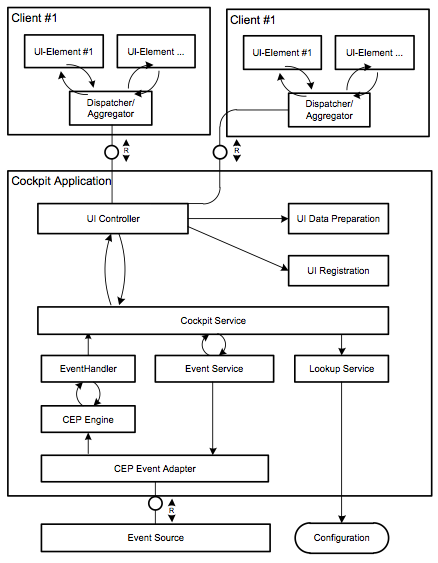
\includegraphics[scale=0.5]{sta.png}
		\caption[System technical architecture]{System technical architecture}
		\label{fig:SystemTechnicalArchitecture}
	\end{center}
\end{figure}

\subsection{The COSM Adapter}
COSM is a online database that offers sensor-data from devices that tracks environment data from objects. It provides an API that allow to push and receive data.
This data is organized in feeds that is specified as a context-specific collection of measurement data - defined by the creator. This feed contains a set of datastreams, each of this represents an individual sensor. Every datastream must have a unique alphanumeric number. It also can define some user-defined tags.

The COSM API currently based in HTTP requests. It conforms with the principles of RESTful . So you are able to use the HTTP verbs to determine a action on a data-object.
GET Retrieves the current state of the object,
PUT : Sets the current state of the object,
POST : Creates a new object and DELETE : Deletes the object.
The data-format is JSON what suited to modern web-based applications.

The service is using a API-Key based authentication that can be send via request header or parameter of the URL. If you create an account on their website, you getting an API-Key witch is full-privileged like you account. It is also possible to request new API-Keys for special feeds that could be managed individually.

The websocket support is listed as a beta-feature in the documentation. With this technique you getting an bi-directional communication socket that allows you to send messages without the HTTP overhead for every message.
Once you are connected to the server, the protocol is wrapped HTTP Request in JSON to send actions to the API. So you are able to use the same GET,PUT,POST and DELETE commands as normal over the HTTP API.

To have a real benefit using the api over the websocket api it is possible to subscribe to every particular feed or datastream you are interested in. When some resource is updated the cosm-server sends immediately datastream representation of the current state via the socket. That enables you to receive real-time push notification about your streams.


\begin{figure}[h]
	\begin{center}
		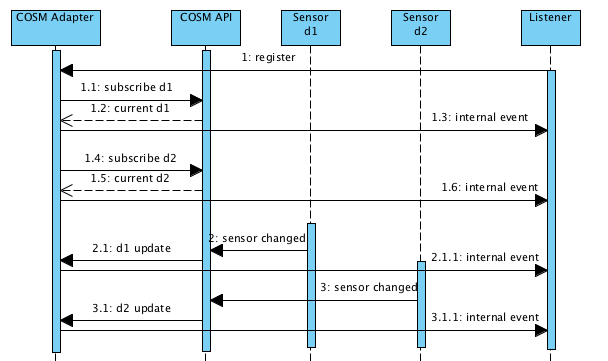
\includegraphics[scale=0.4]{sequence-diagram-cosm.png}
		\caption[Sequence Diagram of the COSM Adapter]{Sequence Diagram of the COSM Adapter}
		\label{fig:SequenceDiagram}
	\end{center}
\end{figure}


So we using a asynchronous http client to register a websocket connection to the cosm api and subscribing us to a list of related datastreams we want to get informed via push.
Once a event is received by the module, it is parsed through a objectmapper to java objects that could be processed. When a change is detected this is pushed via event to other modules that are interested in this information.
To register as an listener for the COSM Adapter it provides a interface that could handle objects that implements the event-listener interface.


\subsection{Complex Event Processing}

The esper engine is loose coupled via the event-listener interface to the cosm-adapter.
These events are filled in the CEP-Engine with a timestamp, numeric data and a target field to define the source sensor.
With this events in the engines database it is possible to define some rules in a Domain Specific Language (DSL) developed by the espertech company and that is called Event Processing Language (EPL). This rules are defined in a sql-like syntax and can define also time windows for time specific definitions.
Once a definition is added to the system engine, every match results in a new event that is thrown by the engine and could be handled by any interested listener.

In our prototype we using this rules to define the business logic for our use-case.
So the cockpit service, that represents our model, is registered as listener by the CEP-Engine and get updates through some special rules that are defined in EPL.
For example we using the raw sensor events from cosm to update our waypoints model.
Also it is possible to refill this created events back into the engine to use them for more high level rules that could be triggered by combinations of complex events.
The ampel system  for a complete route defined in section \ref{sec:Use Case} depends on different events combinations that containing self-defined events.
So we are free to define a arbitrary level of complex events.

\subsection{UI Front-End}
Our front-end, also known as cockpit in this paper, is implemented with state-of-the art browser-based web technologies.
It receives the model via a websocket api that is provided by the cockpit-service.
Every time the backend model is updated, the new model is published by the api and enables the client to react and rebuild or modify the visualization.

As visualization elements we choose a two component view consisting of a table that shows an quick textual overview about the current state and a map that shows the routes on it to offer an other view point of view for this data. Also the route view provides the different routes in the specific ampel-style that is evaluated by the backend.1
As this views are updated in real-time the operator has the possibilities to react very quick to occurred events.

The inner architecture contains an controller that act as dispatcher for incoming events and routes them to the different views. With this architecture it is easy to add more view representations for the backend model without changing any code on the server or disable/enable some view components.
		
\subsection{Wrote a little client to Update the resources via http Request.}

\section{Learning Outcome}
During this project we learned a lot about the future-internet thoughts and the state-of-the-art technologies that are used to realize this ideas.
Due my work beside the university projects i already used some of the technologies where i am developing an monitoring system that also deals with events and visualization of data.

We learned a lot about some future-internet concepts like Internet of Things and Internet of Services and how they used in real world projects. That open us some new views on projects and problems that are currently growing. For many domains this concepts could bring a great benefit for their business cases.

The usage of a Complex-Event-Processing-Engine to deal with business events was a really interesting experience that offers new useful possibilities for other projects i am currently working at. It needs other strategies and approaches to solve this like the definition of an domain specific language for the rules that are defined in these engines.
The usage of an event driven architecture was a good step to use the benefits of every component that deals with real-time events. Also it enabled us to work complete distributed by defining decoupled components. This was a great experience for then whole team because it reduces the effort of many merges and refactoring iterations.

Especially the usage of the websocket protocol with an external api showed me the power but also the problem of these kind of communication protocol. When using the websocket  to communicate you need to define an own inner protocol to handle the messages. 
That could be a wrapped HTTP frame like it is done by COSM or a complete self-designed specification.

In Regular meetings we where able to combine our skills and helped each other through code reviews and analyses of commits. In this point we learned that the usage of a version control system needs some rules that should be clear for all team members. For example a commit should represent a small single task and is tagged with a meaningful commit message that every other team mate could work with this information. The team should define what is a small task and a meaningful commit for this project.

The usage of maven as build management tool was a great choice. After a initial phase of configuration that took a few hours, every teammate could build, pack and start the system per one command at their own development environments. Even our executable package for the appendix is created by one simple command. Including an configured Tomcat with our webapp deployed in it.

Also we learned a lot by working on the front-end design with HTML5 and Javascript.
The usage of javascript what is an functional programming language affords a switch in thinking about problems and how to solve them in a elegant way.
For our project this functional approach was a perfect match to our event driven architecture what enabled us very quick to handle this.
Another great experience was the multi-device support. we tested our application on a normal web-browser and a iPad 3 - it works perfect in both cases.

\section{Conclusion}
\label{sec:Conclusion}
This case study shows that the concepts of the future internet and especially the Internet of Thing concept could be used to solve some problems that occurs in the logistic sector.
This prototype shows the possibilities of such an architecture and technology stack and can be used in various domains with a similar problem. 
We using a sensor network that provides real-time data that is aggregated by COSM Service. This service also provides a websocket api that enables us to get this data in realtime for processing in our application. Inside our application we using the a CEP Engine to combine events an create more meaningful complex events that are used to update our business model. Finally we build a front-end application cockpit that visualizes  this business model.
All these components are build with in an event-driven-architecture that enables us to transport this events in real-time.

There are a lot possibilities to extend and optimize this prototype. We could connect other IoT Platforms to improve the sensor-data input. Also defining more business events for our CEP engine that helps to identify complex event combinations. These could be used for new visualization elements that could be added into the frontend layer.
With our chosen decoupled architecture this extensions would be easy to add into the existing system.

We think that this project has successfully shown that this kind of architecture is a benefit for applications with informational real-time challenges. This first prototype worked very good in our tests. The composition of technologies fits very good together and make it easy to extend for commercial usage. Using HTML5 as technology for the frontend could enable companies to use one implementation for many devices. 
With this prototype as blueprint it is possible to create an valuable software for this kind of domains with related challenges.

%\end{document}  % This is where a 'short' article might terminate

%
% The following two commands are all you need in the
% initial runs of your .tex file to
% produce the bibliography for the citations in your paper.
\bibliographystyle{abbrv}
\bibliography{sigproc}  % sigproc.bib is the name of the Bibliography in this case
% You must have a proper ".bib" file
%  and remember to run:
% latex bibtex latex latex
% to resolve all references
%
% ACM needs 'a single self-contained file'!
%
%APPENDICES are optional
%\balancecolumns
\appendix
%Appendix A
\end{document}
